\documentclass[10pt,pdf,utf8,russian,aspectratio=169]{beamer}
\usepackage{cmap}
\usepackage[T2A]{fontenc}
%\usepackage[utf8x]{inputenc}
\usepackage[russian,english]{babel}
\usepackage{subfig}
\usepackage{graphicx}
\usepackage{multicol}
\usepackage{cancel}
\usepackage{tabularx}
\usepackage{xargs}      
\DeclareSymbolFontAlphabet{\mathbb}{AMSb}%
\DeclareSymbolFontAlphabet{\amsmathbb}{bbold}%

       % AMS Math

%
% Choose how your presentation looks.
%
% For more themes, color themes and font themes, see:
% http://deic.uab.es/~iblanes/beamer_gallery/index_by_theme.html
%
\mode<presentation>
{
  \usetheme{Boadilla}      % or try Darmstadt, Madrid, Warsaw, ...
  \usecolortheme{seagull} % or try albatross, beaver, crane, ..

  \usefonttheme{structurebold}  % or try serif, structurebold, ...
  \setbeamertemplate{navigation symbols}{}
  \setbeamertemplate{caption}[numbered]
} 

\captionsetup[subfloat]{labelformat=empty}
\title[Метаоптимизация и выбор структуры]{Метаоптимизация и структура}
\author{Бахтеев Олег}
\institute{МФТИ}
\date{12.11.2019}
%\renewcommand{\headrulewidth}{0pt}
\DeclareMathOperator*{\argmin}{arg\,min}
\DeclareMathOperator*{\argmax}{arg\,max}
\DeclareUnicodeCharacter{00A0}{ } % При наборе текста с планшета появляются невидимые символы. ЭТо костыль.
\begin{document}
% nb: очень не люблю макросы. Но что поделать 
% https://stackoverflow.com/questions/1509799/how-to-replace-latex-macros-with-their-definitions-using-latex
\newcommand{\D}{\mathfrak{D}}
\newcommand{\x}{\mathbf{x}}
\newcommand{\X}{\mathbf{X}}
\newcommand{\y}{\mathbf{y}}
\newcommand{\Xb}{\mathbb{X}}
\newcommand{\yb}{\mathbb{Y}}
\newcommand{\F}{\mathfrak{F}}



\newcommand{\w}{\mathbf{w}}
\newcommand{\Wb}{\mathbb{W}}
\newcommand{\Uw}{U_\mathbf{w}}

\newcommand{\Gam}{\boldsymbol{\Gamma}}
\newcommand{\Gb}{\amsmathbb{\Gamma}}
\newcommand{\UG}{U_{\boldsymbol{\Gamma}}}

\newcommand{\h}{\mathbf{h}}
\newcommand{\Hb}{\mathbb{H}}
\newcommand{\Uh}{U_{\mathbf{h}}}

\newcommand{\teta}{\boldsymbol{\theta}}
\newcommand{\Tetab}{\amsmathbb{\Theta}}
\newcommand{\Uteta}{U_{\boldsymbol{\theta}}}

\newcommand{\tetaw}{\boldsymbol{\theta}_\mathbf{w}}
\newcommand{\Tetawb}{\amsmathbb{\Theta}_\mathbf{w}}
\newcommand{\Utetaw}{U_{\boldsymbol{\theta}_\mathbf{w}}}
\newcommand{\tetaG}{\boldsymbol{\theta}_{\boldsymbol{\Gamma}}}
\newcommand{\TetaGb}{\amsmathbb{\Theta}_{\boldsymbol{\Gamma}}}
\newcommand{\UtetaG}{U_{\boldsymbol{\theta}_{\boldsymbol{\Gamma}}}}

\newcommand{\lam}{\boldsymbol{\lambda}}
\newcommand{\Lamb}{\amsmathbb{\Lambda}}
\newcommand{\Ulam}{U_{\boldsymbol{\lambda}}}

%\newcommand{\prior}{p(\mathbf{w}, \boldsymbol{\Gamma}|\mathbf{h},\boldsymbol{\lambda})}
\newcommandx{\prior}[4][1=\mathbf{w},2=\boldsymbol{\Gamma},3=\mathbf{h},4=\boldsymbol{\lambda},usedefault]{p(#1,#2|#3,#4)}
\newcommandx{\priorh}[2][1=\mathbf{h}, 2=\boldsymbol{\lambda},usedefault]{p(#1|#2)}
\newcommandx{\priorG}[3][1=\boldsymbol{\Gamma}, 2= \mathbf{h}, 3=\boldsymbol{\lambda},usedefault]{p(#1|#2,#3)}
\newcommandx{\priorw}[4][1=\mathbf{w},2=\boldsymbol{\Gamma},3=\mathbf{h},4=\boldsymbol{\lambda},usedefault]{p(#1|#2,#3,#4)}


\newcommand{\post}{p(\mathbf{w}, \boldsymbol{\Gamma}|\mathbf{y}, \mathbf{X}, \mathbf{h},\boldsymbol{\lambda})}
\newcommand{\posth}{p(\mathbf{h}|\mathbf{y}, \mathbf{X},\boldsymbol{\lambda})}
\newcommand{\postG}{p(\boldsymbol{\Gamma}|\mathbf{y}, \mathbf{X}, \mathbf{h},\boldsymbol{\lambda})}
\newcommand{\postw}{p(\mathbf{w}|\mathbf{y}, \mathbf{X}, \boldsymbol{\Gamma}, \mathbf{h},\boldsymbol{\lambda})}


\newcommandx{\q}[1][1=\boldsymbol{\theta}, usedefault]{q(\mathbf{w}, \boldsymbol{\Gamma}|#1)}
\newcommandx{\qG}[2][1=\boldsymbol{\Gamma},2=\boldsymbol{\theta}_{\boldsymbol{\Gamma}},usedefault]{q_{\boldsymbol{\Gamma}}(#1|#2)}
\newcommandx{\qw}[3][1=\mathbf{w}, 2=\boldsymbol{\Gamma},3=\boldsymbol{\theta}_\mathbf{w},usedefault]{q_\mathbf{w}(#1|#2,#3)}


\newcommandx{\LL}[4][1=\mathbf{y},2=\mathbf{X},3=\mathbf{w},4=\boldsymbol{\Gamma},usedefault]{p(#1|#2,#3,#4)}

\newcommand{\EV}{p(\mathbf{y}|\mathbf{X}, \mathbf{h},\boldsymbol{\lambda})}

\newcommandx{\Loss}[5][1=\boldsymbol{\theta},2=\mathbf{y},3=\mathbf{X},4=\mathbf{h},5=\boldsymbol{\lambda},usedefault]{L(#1 |#2,#3,#4,#5)}
\newcommandx{\Val}[5][1=\mathbf{h},2=\mathbf{y},3=\mathbf{X},4=\boldsymbol{\theta},5=\boldsymbol{\lambda},usedefault]{Q(#1|#2,#3,#4,#5)}

% прочее
\newcommand{\model}{\mathbf{f}}
\newcommand{\A}{\mathbf{A}}
\newcommand{\s}{\mathbf{s}}
\newcommand{\g}{\boldsymbol{\gamma}}
\newcommand{\E}{\mathsf{E}}
\newcommand{\KL}[2]{D_\text{KL}\bigl(#1 || #2\bigr)}

\newcommand{\lamT}{\lambda_{\text{temp}}}
\newcommand{\lamLL}{\lambda_\text{likelihood}^\text{Q}}
\newcommand{\lamCL}{\lambda_\text{prior}^\text{L}}
\newcommand{\lamCQ}{\lambda_\text{prior}^\text{Q}}
\newcommand{\lamS}{\boldsymbol{\lambda}_\text{struct}^\text{Q}}
\newcommandx{\TLoss}[6][1=\boldsymbol{\theta},2=L,3=\mathbf{y}, 4=\mathbf{X}, 5=\mathbf{h},6=\boldsymbol{\lambda},usedefault]{T(#1|#2,#3,#4,#5,#6)}
\newcommandx{\TVal}[6][1=\mathbf{h},2=Q,3=\mathbf{y}, 4=\mathbf{X}, 5=\boldsymbol{\teta},6=\boldsymbol{\lambda},usedefault]{T(#1|#2,#3,#4,#5,#6)}
%\newcommand{\log}{\text{log}~}




\begin{frame}
  \titlepage
\end{frame}

\begin{frame}{В предыдущих сериях: гиперпараметры}
\begin{block}{Определение}
Априорным распределением $p(\mathbf{w}|\mathbf{h})$ параметров модели назовем вероятностное распределение, соответствующее предположениям о
распределении параметров модели.
\end{block}

\begin{block}{Определение}
Гиперпараметрами $\mathbf{h} \in \mathbb{H}$ модели назовем параметры априорного распределения (параметры распределения параметров модели).
\end{block}

\end{frame}



\begin{frame}{В предыдущих сериях: гиперпараметры}
Задана дифференцируемая по параметрам модель, приближающая зависимую переменную~$y$:
\[
	\mathbf{f}:\mathbb{R}^n \to \mathbb{Y}, \quad \mathbf{w} \in \mathbb{R}^u.
\]
Функция $\mathbf{f}$ задает правдоподобие выборки $\text{log}p(\mathbf{y}|\mathbf{X}, \mathbf{w})$. 

Пусть также задано априорное распределение параметров $p(\mathbf{w}|\mathbf{h})$.
\vspace{1cm}

\textbf{Пример:}
 $$\mathbf{w} \sim \mathcal{N}(\mathbf{0}, \mathbf{A}^{-1}),$$
где $\mathbf{A}^{-1} = \text{diag}[\alpha_1, \dots, \alpha_u]^{-1}$ --- матрица ковариаций диагонального вида, определяемая \textit{гиперпараметрами} $[\alpha_1, \dots, \alpha_u] = \mathbf{h}$. 
\end{frame}

\begin{frame}{В предыдущих сериях: гиперпараметры}
Пусть $\boldsymbol{\theta} \in \mathbb{R}^s$ --- множество всех оптимизируемых параметров.\\
$L(\boldsymbol{\theta},\mathbf{h})$ ---  дифференцируемая функция потерь  по которой производится оптимизация функции $\mathbf{f}$. \\
$Q(\boldsymbol{\theta},\mathbf{h})$ ---  дифференцируемая функция определяющая итоговое качество модели $\mathbf{f}$ и приближающая интеграл.\\

Требуется найти параметры ${\boldsymbol{\theta}}^{*}$ и гиперпараметры ${\mathbf{h}}^{*}$ модели, доставляющие минимум следующему функционалу:
\[
{\mathbf{h}}^{*} = \argmax_{\mathbf{h} \in \mathbb{H}} Q({\boldsymbol{\theta}^{*}}(\mathbf{h}), \mathbf{h}),
\]
\[
	{\boldsymbol{\theta}}(\mathbf{h})^{*} =  \argmin_{\boldsymbol{\theta} \in \mathbb{R}^s} L(\boldsymbol{\theta}, \mathbf{h}).
\]
\end{frame}

\begin{frame}{В предыдущих сериях: вариационная оценка}
\textbf{Вариационная оценка Evidence}, Evidence lower bound --- метод нахождения приближенного значения аналитически невычислимого распределения $p(\mathbf{w}|\mathfrak{D}, \mathbf{h})$ распределением $q(\mathbf{w}) \in \mathfrak{Q}$. Получение вариационной нижней оценки обычно сводится к задаче минимизации
$$\text{KL}(q(\mathbf{w})||p(\mathbf{w}| \mathfrak{D}))=
-\int_{\mathbf{w}} q(\mathbf{w}) \text{log}~\frac{p(\mathbf{w}| \mathfrak{D})} {q(\mathbf{w})}d\mathbf{w} = \textcolor{blue}{\mathsf{E}_{\mathbf{w}} \text{log}~p(\mathfrak{D}|\mathbf{w})} - \textcolor{red}{\text{KL}(q(\mathbf{w})||p(\mathbf{w}| \mathbf{h}))}.
$$

\textbf{Частным случаем} вариационного распределения можно считать распределение параметров модели под действием оптимизации.
\end{frame}


\begin{frame}{Метапараметры}
\begin{block}{Wikipedia}
A parameter that controls the value of one or more others.
\end{block}

\begin{block}{Определение}
Метапараметрами $\boldsymbol{\lambda}$ модели назовем параметры оптимизации.
\end{block}

Чаще всего метапараметры назначаются экспертно и не подлежат оптимизации в ходе решения задачи выбора модели. 

Что можно считать метапараметрами:
\begin{itemize}
\item параметры оператора оптимизации;
\item параметры задачи оптимизации;
\item структуру модели;
\item функции активации слоев сети;
\item вид априорного распределения и функции правдоподобия.
\end{itemize}
\end{frame}


\begin{frame}{A neural network that embeds its own meta-levels}
Предлагается разделить подмодели внутри модели сети по назначениям:
\begin{itemize}
\item ``Normal'' model: обучение и вывод.
\item Evaluation model: оценка качества $Q$.
\item Analyzing model: анализ параметров модели.
\item Modifiyng model: модификация параметров.
\end{itemize}

Представлен градиентный алгоритм оптимизации нейронной сети.
\end{frame}



\begin{frame}{Learning to learn by gradient descent by gradient descent}
\textbf{Идея: } рассматривать оператор оптимизации $T$ как дифференцируемую функцию:
\[
    T(\boldsymbol{\theta}) = \text{LSTM}(\boldsymbol{\theta}).
\]
Оптимизационная задача:
\[
    \sum_{t=t_0}^{t_\eta} L\left(T^t(\boldsymbol{\theta}_{t_0})\right) \to \max.
\]

LSTM имеет небольшое число параметров и делит параметры между всеми метапараметрами оператора.

\begin{figure}
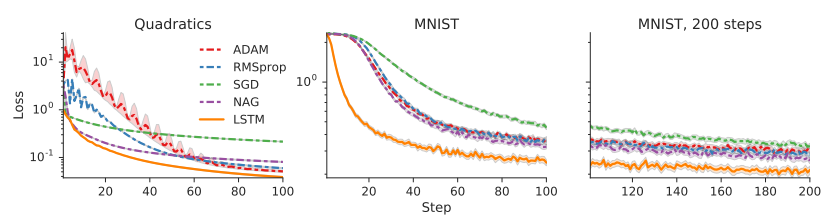
\includegraphics[width=\textwidth]{sgd_by_sgd.png}
\end{figure}
\end{frame}


\begin{frame}{Optimal Brain Damage}
Рассматривается задача удаления неинформативных параметров.

\textbf{Идея метода:}
Разложим функцию потерь в ряд Тейлора в окрестности максимума $\boldsymbol{\theta}^{*}:$
\[
    L(\boldsymbol{\theta}^{*} + \Delta \boldsymbol{\theta}) -  L(\boldsymbol{\theta}^{*} ) = -\frac{1}{2} \boldsymbol{\theta} \mathbf{H} \boldsymbol{\theta}  + o(||\Delta \boldsymbol{\theta}||^3),
\]
где $\mathbf{H}$ --- гессиан функции $-L$.

Для простоты вычисления будем полагать гессиан диагональным. Задача удаления параметров сводится к рассмотрению задач условной оптимизации вида:
\[
    L(\boldsymbol{\theta}^{*} + \Delta \boldsymbol{\theta}) \to \max 
\]
при 
\[
    {\theta}^{*}_i + \Delta \theta_i = 0.
\]

Показатель информативности параметра: 
\[
    \frac{\theta_{i}^2}{2[\mathbf{H}^{-1}]_{i,i}}.
\]

\end{frame}


\begin{frame}{Learning both Weights and Connections for Efficient Neural Networks}
\textbf{Идея подхода:}
\begin{enumerate}
\item Оптимизируем модель;
\item Удаляем наименьшие по модулю параметры;
\item Запускаем оптимизацию заново.
\end{enumerate}

Почти очевидные факты, которые подтверждаются в статье:
\begin{itemize}
\item $L_2$ лучше для прунинга, чем $L_1$ в случае, если после прунинга идет оптимизация.
\item Оптимизацию лучше производить из предыдущего оптимума, чем из случайной точки.
\item После прунинга распределение параметров становится мультимодальным.
\end{itemize}
\begin{figure}
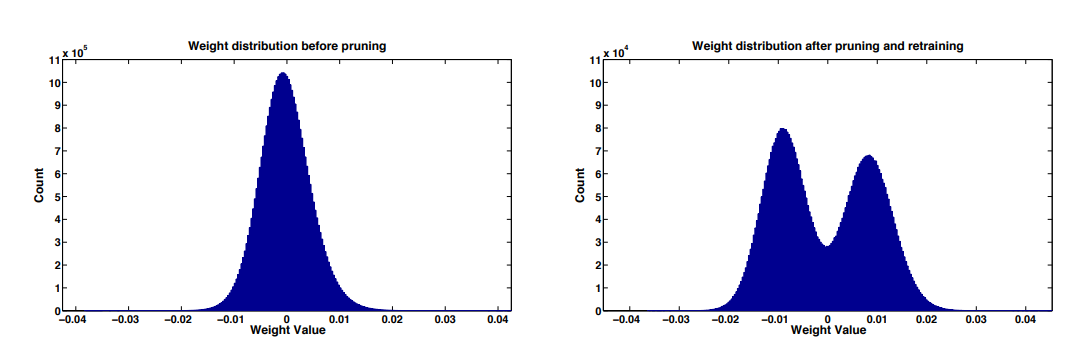
\includegraphics[width=0.75\textwidth]{bimodal.png}
\end{figure}


\end{frame}


\begin{frame}{Deep Compression}
\textbf{Идея подхода:}
\begin{enumerate}
\item Удаляем ненужные параметры модели, аналогично предыдущем подходу.
\item Кластеризуем параметры (K-means на каждом слое).
\item Производим повторную оптимизацию на центроидах.
\item Кодируем индексы параметров с использованием кодов Хаффмана.
\end{enumerate}

Результат: уменьшение размеров модели в 40 раз, ускорение в 3 раза.
\begin{figure}
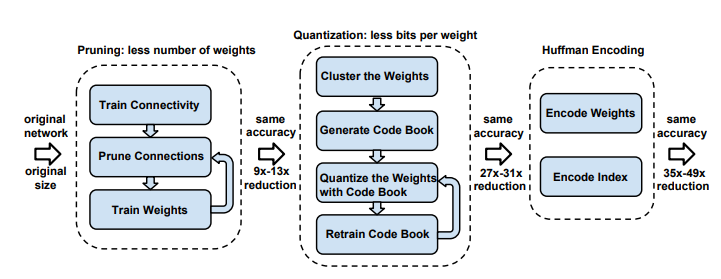
\includegraphics[width=0.75\textwidth]{huffman.png}
\end{figure}

\end{frame}


\begin{frame}{Graves, 2011}
\small
\[
\text{MDL}(\mathbf{f}, \mathfrak{D}) = L(\mathbf{f}) + L(\mathfrak{D}|\mathbf{f}),
\]
где $\mathbf{f}$ --- модель, $\mathfrak{D}$ --- выборка, $L$ --- длина описания в битах.
\\
\[
\text{MDL}(\mathbf{f}, \mathfrak{D}) \sim L(\mathbf{f}) + \textcolor{blue}{L(\mathbf{w}^*| \mathbf{f})} + \textcolor{red}{L(\mathfrak{D}|\mathbf{w}^*, \mathbf{f})},
\]
$\mathbf{w}^*$ --- оптимальные параметры модели.\\


$$
L =   \textcolor{blue}{\sum_{\mathbf{x}, \mathbf{y}} \text{log}~p(\mathbf{y}|\mathbf{x}, \hat{\mathbf{w}})} + \textcolor{red}{\frac{1}{2} \bigl( \text{tr} (\mathbf{A}_q) + \boldsymbol{\mu}_q^\text{T}\mathbf{A}^{-1}\boldsymbol{\mu}_q  - \text{ln}~|\mathbf{A}_q| \bigr)}.
$$


Прунинг параметра ${w}_i$ определяется относительной плотностью:
\[
	\lambda = \frac{q(\mathbf{0})}{q(\boldsymbol{\mu}_{i,q})}  = \text{exp}(-\frac{\mu_i^2}{2\sigma_i^2}).
\]
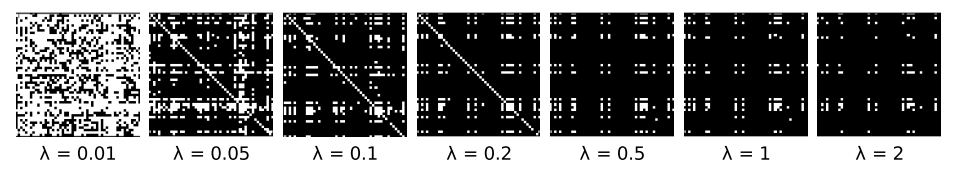
\includegraphics[width=\textwidth]{graves.png}

\end{frame}


\begin{frame}{Bayesian Compression for Deep Learning}
\textbf{Модель 1:}
\[
    \mathbf{z} \sim p(\mathbf{z}); \mathbf{w} \sim \mathcal{N}(0; \mathbf{z}^2),
\]
где $z$ поставлено в соответствие группе параметров (пример: нейронам).

Априорное распределение $p(z) \propto \frac{1}{|z|^2}$.

Вариационное распределение: 
$
    \mathbf{z} \sim \mathcal{N}(\boldsymbol{\mu}_z, \boldsymbol{\sigma}_z), \mathbf{w} \sim  \mathcal{N}(\boldsymbol{\mu}, \boldsymbol{\sigma})
$ 

Критерий удаления параметров:
\[
    \text{log}~{\sigma_z} - \text{log}~{\mu_z} > \lambda.
\]


\end{frame}


\begin{frame}{Bayesian Compression for Deep Learning}
\textbf{Модель 2:}
Априорное распределение:
\[
   s \sim C^{+} (0, \lambda_0), z_i  \sim C^{+} (0, 1), \hat{w_{i,j}} \sim \mathcal{N}(0,1),  w_{i,j} =  s  z_i \hat{w_{i,j}}.
\]

Вариационное распределение для $z_i$: 
$
    \mathbf{z}_i \sim  \mathcal{LogN} (\boldsymbol{\mu}, \boldsymbol{\sigma}) \mathcal{LogN} (\boldsymbol{\mu}_i, \boldsymbol{\sigma}_i)
$ 


\begin{figure}
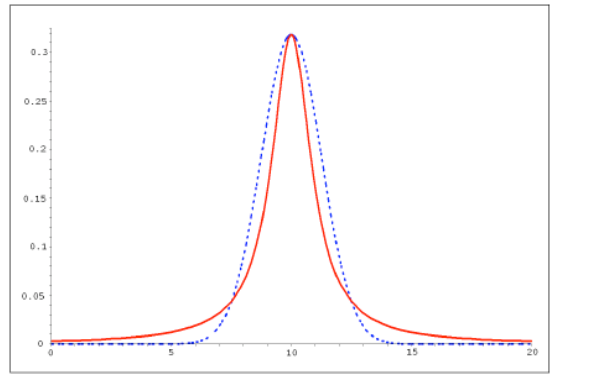
\includegraphics[width=0.5\textwidth]{cauchy.png}
\caption*{[Comparing the Cauchy and Gaussian (Normal) density functions, F. Masci]}
\end{figure}
\end{frame}


\begin{frame}{Learning the structure of deep sparse graphical models}
Рассматривается глубокая генеративная модель.

Структура (т.е. связи параметров) сэмплируются в соответствии с распределением Индийского буфета. Интерпретация распределения:
\textit{В ресторане находится конечное количество клиентов и бесконечное количество блюд. $j$-й клиент берет блюдо $k$ с вероятностью:
\[
    \frac{\eta_k}{j+\beta-1},
\]
где $\eta_k$ количество выборов этого блюда предыдщими клиентами (популярность блюда), а также несколько новых блюд в соответствии с рапределением Пуассона с параметром $\frac{\alpha \beta }{j+\beta - 1}$.}

Порождение параметров и структуры происходит с помощью MCMC.


\textbf{Главный вывод:} структуру можно рассматривать как случайную величину и применять вероятностные методы.

\end{frame}




\begin{frame}{Learning the structure of deep sparse graphical models}
\begin{figure}
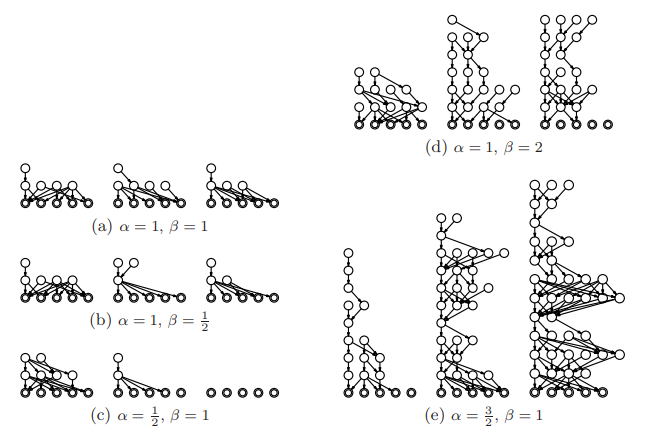
\includegraphics[width=0.75\textwidth]{buffet.png}
\end{figure}

\end{frame}

\begin{frame}{Вид вариационной оценки}
Обозначим структуру $\boldsymbol{\Gamma}$.
Пусть априорное распределение параметров зависит от структуры:
$$\mathbf{w} \sim p(\mathbf{w}|\boldsymbol{\Gamma}, \mathbf{h}), \quad \mathbf{w} \sim^q q(\mathbf{w}|\boldsymbol{\Gamma})$$

Тогда вариационная оценка имеет вид:
\[
    \mathsf{E}_q \text{log}p(\mathbf{y}|\mathbf{x}, \mathbf{w}, \boldsymbol{\Gamma}) - \text{KL}\left(q(\boldsymbol{\Gamma})||p(\boldsymbol{\Gamma}|\mathbf{h})\right) - \mathsf{E}_{\boldsymbol{\Gamma} \sim q(\boldsymbol{\Gamma})}\text{KL} \left (q(\mathbf{w}|\boldsymbol{\Gamma})||p(\mathbf{w}|\boldsymbol{\Gamma}, \mathbf{h})\right).
\]
\end{frame}


\begin{frame}{Параметрическая сложность}
Относительной вариационной   плотностью  назовем отношение:
\[
\rho(w| \mathbf{h})=\frac{q_\mathbf{w}(\text{mode}~p(\mathbf{w}|\boldsymbol{\Gamma}, \mathbf{h}, \boldsymbol{\lambda}))}{q_\mathbf{w}(\text{mode}~{q_\mathbf{w}})},\quad  \boldsymbol{\rho} = \prod_{w \in \mathbf{w}} \rho(w|\boldsymbol{\Gamma},\boldsymbol{\theta}_\mathbf{w}, \mathbf{h},\boldsymbol{\lambda}).
\]

\begin{block}{Определение}
Параметрической сложностью модели назовем минимальную дивергенцию между априорным и вариационным распределением:
\vspace{-0.2cm}
\[
    C_p = \min_{\mathbf{h} \in U} \textcolor{red}{D_\text{KL}(q||p(\mathbf{w}, \boldsymbol{\Gamma}|\mathbf{h},\lambda_\text{temp}, \mathbf{f})),}
\]
где $U$ --- некоторый компакт.
\end{block}
\vspace{-0.2cm}
\begin{block}{Утверждение}
Пусть задана последовательность
$\boldsymbol{\theta}[1],\boldsymbol{\theta}[2], \dots$, такая, что $\lim_{i \to \infty}C_p(\boldsymbol{\theta}[i]) = 0.$
Тогда:
\footnotesize
$$
   \lim_{i \to \infty} \mathsf{E}_{q(\boldsymbol{\Gamma})} \boldsymbol{\rho}^{-1} (\mathbf{w}|\mathbf{h}[i]) = 1,
$$
где $\mathbf{h} = \argmin_{\mathbf{h} \in U} \textcolor{red}{D_\text{KL}(q||p(\mathbf{w}, \boldsymbol{\Gamma}|\mathbf{h},\lambda_\text{temp}, \mathbf{f}))}$
\end{block}

\end{frame}


\begin{frame}{Обобщающая задача оптимизации}
Какие требования можно выдвинуть к ``хорошей'' функции оптимизации?
\begin{enumerate}
\item При некоторых значениях метапараметров функция должна приближать \textcolor{blue}{метод максимального правдоподобия}.
\item При некоторых значениях метапараметров функция должна штрафовать \textcolor{red}{излишне сложные модели.}
\item При некоторых значениях метапараметров функция должна приближать обоснованность модели.
\item При некоторых значениях метапараметров функция должна позволять \textcolor{olive}{переходить между оптимальными структурами модели.}
\item Функции потерь и валидации должны быть непрерывны по метапараметрам.
\item Область определения функции должна быть нетривиальна.
\end{enumerate}
\end{frame}

\begin{frame}{Критерии перехода между структурами}
\small
\begin{block}{критерий 1}
Существует нетривиальная константа $K$ и метапараметры $\boldsymbol{\lambda}$, такие что для любой пары локальных оптимумов $\mathbf{h}_1, \mathbf{h}_2$ и соответствующих им вариационных параметров $\boldsymbol{\theta}(\mathbf{h}_1), \boldsymbol{\theta}(\mathbf{h}_2)$, таких что $\text{KL}(q(\boldsymbol{\Gamma}|\boldsymbol{\theta}_1)||q(\boldsymbol{\Gamma}|\boldsymbol{\theta}_2))>K, \text{KL}(q(\boldsymbol{\Gamma}|\boldsymbol{\theta}_2)||q(\boldsymbol{\Gamma}|\boldsymbol{\theta}_1))>K$ и $Q(\mathbf{h}_1|\boldsymbol{\lambda}) > Q(\mathbf{h}_2|\boldsymbol{\lambda})$,  существует значение $\boldsymbol{\lambda}'$, такое что:
\begin{enumerate}
\item соответствия $\boldsymbol{\theta}(\mathbf{h}_1), \boldsymbol{\theta}(\mathbf{h}_2)$ сохраняются;
\item $Q(\mathbf{h}_1|\boldsymbol{\lambda}) < Q(\mathbf{h}_2|\boldsymbol{\lambda}).$
\end{enumerate}
\end{block}

\begin{block}{Критерий 2}
Существует нетривиальная константа $K$ и метапараметры $\boldsymbol{\lambda}$, такие что для любой пары локальных оптимумов $\mathbf{h}_1, \mathbf{h}_2$ и соответствующих им вариационных параметров $\boldsymbol{\theta}(\mathbf{h}_1), \boldsymbol{\theta}(\mathbf{h}_2)$, таких что $\text{KL}(p(\boldsymbol{\Gamma}|\mathbf{h}_1)||p(\boldsymbol{\Gamma}|\mathbf{h}_2))>K, \text{KL}(p(\boldsymbol{\Gamma}|\mathbf{h}_2)||p(\boldsymbol{\Gamma}|\mathbf{h}_1))>K$ и $Q(\mathbf{h}_1|\boldsymbol{\lambda}) > Q(\mathbf{h}_2|\boldsymbol{\lambda})$,  существует значение $\boldsymbol{\lambda}'$, такое что:
\begin{enumerate}
\item соответствия $\boldsymbol{\theta}(\mathbf{h}_1), \boldsymbol{\theta}(\mathbf{h}_2)$ сохраняются;
\item $Q(\mathbf{h}_1|\boldsymbol{\lambda}) < Q(\mathbf{h}_2|\boldsymbol{\lambda}).$
\end{enumerate}
\end{block}

Для $L = Q $ --- вариационной нижней оценки критерий 2 не выполняется.
\end{frame}

\begin{frame}{ДЗ: выбор задания}
\textbf{Дедлайн: 30 октября, 0 часов.}\\~\\

\texttt{ from zlib import crc32}\\~\\
\texttt{theory = crc32('фамилия кириллицей'.lower().encode('utf-8'))\%4+1}\\~\\
\texttt{practice = crc32('фамилия латиницей'.lower().encode('utf-8'))\%3+1}\\~\\

Задания заливаются на github:
\textit{https://github.com/Intelligent-Systems-Phystech/model\_selection/фамилия латиницей}\\

\end{frame}


\begin{frame}{ДЗ: теория}
\textbf{Формат: tex + pdf.}
Задание 1: доказать вид вариационной функции при структуре $\boldsymbol{\Gamma}$ (расписать дивергенцию).
\end{frame}


\begin{frame}{ДЗ: теория}
\textbf{Формат: tex + pdf.}
Задание 2: доказать утверждение
\begin{block}
\iffalse
Пусть
\begin{enumerate}

\item Заданы компактные множества $\Uh \subset \Hb, \Utetaw \subset \Tetawb, \UtetaG \subset \TetaGb$.

\item Вариационное распределение $\qw$  является абсолютно непрерывным и унимодальным на  $U_{\boldsymbol{\theta}}$.
Его мода и матожидание совпадают:

\[
  \text{mode}~\qw = \E_{\qw} \w.
\]




\item Априорное распределение $\priorw$ является абсолютно непрерывным и унимодальным на  $U_\mathbf{h}$. Его мода и матожидание совпадают и не зависят от гиперпараметров $\h$  на $\Uh$ и структуры $\Gamma$ на $\UtetaG$:
\[
\E_{\priorw}~\w = \text{mode}~\priorw[][\Gamma_1][\h_1]=\text{mode}~\priorw[][\Gamma_1][\h_2]=\mathbf{m}
\]
\text{ для любых }$~\h_1,\h_2 \in \Uh, \Gamma_1,\Gamma_2 \in \UG$.


\item Параметры модели $\w$ имеют конечные вторые моменты по маргинальным распределениям:
\[
   \int_{\Gamma}\qG\qw d\Gamma, \quad \int_{\Gamma}\qG\priorw d\Gamma
\]
при любых $\tetaw \in \Utetaw, \tetaG \in \UtetaG, \h \in \Uh.$


\item Вариационное распределение $\qw$ является липшицевым по $\w$.

\item Значение $\qw$ не равно нулю при любых $\teta \in \Uteta, \Gamma \in \Gb$.

\item Точная нижняя грань $\qw[\mathbf{m}]$ не равна нулю при $\tetaw \in \Utetaw$ и $\Gamma \in \Gb$:
\[
    \inf_{\Gamma \in \Gb, \tetaw \in \Utetaw} \qw[\mathbf{m}] > 0.
\]
\end{enumerate}
Тогда 
\[
   \left|\E_{\qG} {\rho}(\w|\Gamma, \tetaw, \h, \lam)^{-1} - 1\right| \leq
\]
\[
\leq \frac{C_l}{\inf_{\Gamma' \in \Gb, \tetaw' \in \Utetaw} \qw[\mathbf{m}][\Gamma'][\tetaw']} \iint_{\Gamma,\w} |\w| \cdot |\qw - \priorw|\qG d\w d\Gamma,
\]
где $C_l$ --- максимальная константа Липшица для $\qw$ на $\Uteta$.
\fi
\end{block}
\end{frame}


\begin{frame}{ДЗ: практика}
\textbf{Формат: ipynb.}
Реализовать пример оптимизации гиперпараметров на небольшой выборке с ошибкой на валидации в качестве функции $Q$.

Количество гиперпараметров: не менее 20.

Рассмотреть алгоритмы: случайный поиск, гауссовый процесс (библиотечная реализация) и:
\begin{enumerate}
\item HOAG;

\item Жадный алгоритм.

\end{enumerate}

При оценивании будут учитываться аккуратность кода ноутбуков и наглядность примера.\\~\\
Пример должен быть выполнен на  \textbf{простых} игрушечных синтетических данных.
\end{frame}


\begin{frame}
\frametitle{Используемые материалы}
\begin{enumerate}
\item TODO
\end{enumerate}
\end{frame}
\end{document}
